\documentclass[1p]{elsarticle_modified}
%\bibliographystyle{elsarticle-num}

%\usepackage[colorlinks]{hyperref}
%\usepackage{abbrmath_seonhwa} %\Abb, \Ascr, \Acal ,\Abf, \Afrak
\usepackage{amsfonts}
\usepackage{amssymb}
\usepackage{amsmath}
\usepackage{amsthm}
\usepackage{scalefnt}
\usepackage{amsbsy}
\usepackage{kotex}
\usepackage{caption}
\usepackage{subfig}
\usepackage{color}
\usepackage{graphicx}
\usepackage{xcolor} %% white, black, red, green, blue, cyan, magenta, yellow
\usepackage{float}
\usepackage{setspace}
\usepackage{hyperref}

\usepackage{tikz}
\usetikzlibrary{arrows}

\usepackage{multirow}
\usepackage{array} % fixed length table
\usepackage{hhline}

%%%%%%%%%%%%%%%%%%%%%
\makeatletter
\renewcommand*\env@matrix[1][\arraystretch]{%
	\edef\arraystretch{#1}%
	\hskip -\arraycolsep
	\let\@ifnextchar\new@ifnextchar
	\array{*\c@MaxMatrixCols c}}
\makeatother %https://tex.stackexchange.com/questions/14071/how-can-i-increase-the-line-spacing-in-a-matrix
%%%%%%%%%%%%%%%

\usepackage[normalem]{ulem}

\newcommand{\msout}[1]{\ifmmode\text{\sout{\ensuremath{#1}}}\else\sout{#1}\fi}
%SOURCE: \msout is \stkout macro in https://tex.stackexchange.com/questions/20609/strikeout-in-math-mode

\newcommand{\cancel}[1]{
	\ifmmode
	{\color{red}\msout{#1}}
	\else
	{\color{red}\sout{#1}}
	\fi
}

\newcommand{\add}[1]{
	{\color{blue}\uwave{#1}}
}

\newcommand{\replace}[2]{
	\ifmmode
	{\color{red}\msout{#1}}{\color{blue}\uwave{#2}}
	\else
	{\color{red}\sout{#1}}{\color{blue}\uwave{#2}}
	\fi
}

\newcommand{\Sol}{\mathcal{S}} %segment
\newcommand{\D}{D} %diagram
\newcommand{\A}{\mathcal{A}} %arc


%%%%%%%%%%%%%%%%%%%%%%%%%%%%%5 test

\def\sl{\operatorname{\textup{SL}}(2,\Cbb)}
\def\psl{\operatorname{\textup{PSL}}(2,\Cbb)}
\def\quan{\mkern 1mu \triangleright \mkern 1mu}

\theoremstyle{definition}
\newtheorem{thm}{Theorem}[section]
\newtheorem{prop}[thm]{Proposition}
\newtheorem{lem}[thm]{Lemma}
\newtheorem{ques}[thm]{Question}
\newtheorem{cor}[thm]{Corollary}
\newtheorem{defn}[thm]{Definition}
\newtheorem{exam}[thm]{Example}
\newtheorem{rmk}[thm]{Remark}
\newtheorem{alg}[thm]{Algorithm}

\newcommand{\I}{\sqrt{-1}}
\begin{document}

%\begin{frontmatter}
%
%\title{Boundary parabolic representations of knots up to 8 crossings}
%
%%% Group authors per affiliation:
%\author{Yunhi Cho} 
%\address{Department of Mathematics, University of Seoul, Seoul, Korea}
%\ead{yhcho@uos.ac.kr}
%
%
%\author{Seonhwa Kim} %\fnref{s_kim}}
%\address{Center for Geometry and Physics, Institute for Basic Science, Pohang, 37673, Korea}
%\ead{ryeona17@ibs.re.kr}
%
%\author{Hyuk Kim}
%\address{Department of Mathematical Sciences, Seoul National University, Seoul 08826, Korea}
%\ead{hyukkim@snu.ac.kr}
%
%\author{Seokbeom Yoon}
%\address{Department of Mathematical Sciences, Seoul National University, Seoul, 08826,  Korea}
%\ead{sbyoon15@snu.ac.kr}
%
%\begin{abstract}
%We find all boundary parabolic representation of knots up to 8 crossings.
%
%\end{abstract}
%\begin{keyword}
%    \MSC[2010] 57M25 
%\end{keyword}
%
%\end{frontmatter}

%\linenumbers
%\tableofcontents
%
\newcommand\colored[1]{\textcolor{white}{\rule[-0.35ex]{0.8em}{1.4ex}}\kern-0.8em\color{red} #1}%
%\newcommand\colored[1]{\textcolor{white}{ #1}\kern-2.17ex	\textcolor{white}{ #1}\kern-1.81ex	\textcolor{white}{ #1}\kern-2.15ex\color{red}#1	}

{\Large $\underline{11a_{315}~(K11a_{315})}$}

\setlength{\tabcolsep}{10pt}
\renewcommand{\arraystretch}{1.6}
\vspace{1cm}\begin{tabular}{m{100pt}>{\centering\arraybackslash}m{274pt}}
\multirow{5}{120pt}{
	\centering
	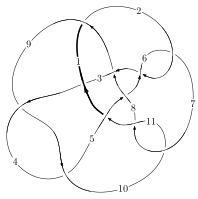
\includegraphics[width=112pt]{../../../GIT/diagram.site/Diagrams/png/564_11a_315.png}\\
\ \ \ A knot diagram\footnotemark}&
\allowdisplaybreaks
\textbf{Linearized knot diagam} \\
\cline{2-2}
 &
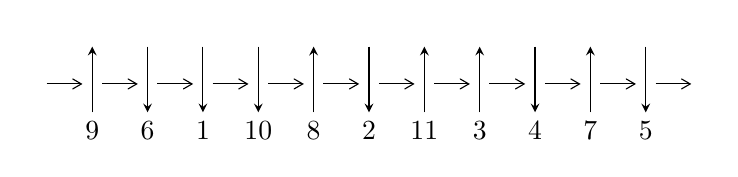
\begin{tikzpicture}[x=20pt, y=17pt]
	% nodes
	\node (C0) at (0, 0) {};
	\node (C1) at (1, 0) {};
	\node (C1U) at (1, +1) {};
	\node (C1D) at (1, -1) {9};

	\node (C2) at (2, 0) {};
	\node (C2U) at (2, +1) {};
	\node (C2D) at (2, -1) {6};

	\node (C3) at (3, 0) {};
	\node (C3U) at (3, +1) {};
	\node (C3D) at (3, -1) {1};

	\node (C4) at (4, 0) {};
	\node (C4U) at (4, +1) {};
	\node (C4D) at (4, -1) {10};

	\node (C5) at (5, 0) {};
	\node (C5U) at (5, +1) {};
	\node (C5D) at (5, -1) {8};

	\node (C6) at (6, 0) {};
	\node (C6U) at (6, +1) {};
	\node (C6D) at (6, -1) {2};

	\node (C7) at (7, 0) {};
	\node (C7U) at (7, +1) {};
	\node (C7D) at (7, -1) {11};

	\node (C8) at (8, 0) {};
	\node (C8U) at (8, +1) {};
	\node (C8D) at (8, -1) {3};

	\node (C9) at (9, 0) {};
	\node (C9U) at (9, +1) {};
	\node (C9D) at (9, -1) {4};

	\node (C10) at (10, 0) {};
	\node (C10U) at (10, +1) {};
	\node (C10D) at (10, -1) {7};

	\node (C11) at (11, 0) {};
	\node (C11U) at (11, +1) {};
	\node (C11D) at (11, -1) {5};
	\node (C12) at (12, 0) {};

	% arrows
	\draw[->,>={angle 60}]
	(C0) edge (C1) (C1) edge (C2) (C2) edge (C3) (C3) edge (C4) (C4) edge (C5) (C5) edge (C6) (C6) edge (C7) (C7) edge (C8) (C8) edge (C9) (C9) edge (C10) (C10) edge (C11) (C11) edge (C12) ;	\draw[->,>=stealth]
	(C1D) edge (C1U) (C2U) edge (C2D) (C3U) edge (C3D) (C4U) edge (C4D) (C5D) edge (C5U) (C6U) edge (C6D) (C7D) edge (C7U) (C8D) edge (C8U) (C9U) edge (C9D) (C10D) edge (C10U) (C11U) edge (C11D) ;
	\end{tikzpicture} \\
\hhline{~~} \\& 
\textbf{Solving Sequence} \\ \cline{2-2} 
 &
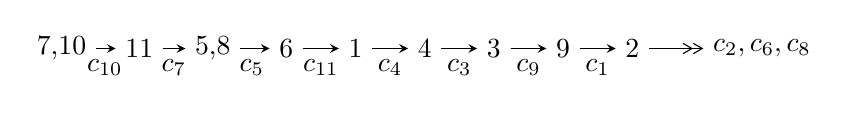
\begin{tikzpicture}[x=25pt, y=7pt]
	% node
	\node (A0) at (-1/8, 0) {7,10};
	\node (A1) at (1, 0) {11};
	\node (A2) at (33/16, 0) {5,8};
	\node (A3) at (25/8, 0) {6};
	\node (A4) at (33/8, 0) {1};
	\node (A5) at (41/8, 0) {4};
	\node (A6) at (49/8, 0) {3};
	\node (A7) at (57/8, 0) {9};
	\node (A8) at (65/8, 0) {2};
	\node (C1) at (1/2, -1) {$c_{10}$};
	\node (C2) at (3/2, -1) {$c_{7}$};
	\node (C3) at (21/8, -1) {$c_{5}$};
	\node (C4) at (29/8, -1) {$c_{11}$};
	\node (C5) at (37/8, -1) {$c_{4}$};
	\node (C6) at (45/8, -1) {$c_{3}$};
	\node (C7) at (53/8, -1) {$c_{9}$};
	\node (C8) at (61/8, -1) {$c_{1}$};
	\node (A9) at (10, 0) {$c_{2},c_{6},c_{8}$};

	% edge
	\draw[->,>=stealth]	
	(A0) edge (A1) (A1) edge (A2) (A2) edge (A3) (A3) edge (A4) (A4) edge (A5) (A5) edge (A6) (A6) edge (A7) (A7) edge (A8) ;
	\draw[->>,>={angle 60}]	
	(A8) edge (A9);
\end{tikzpicture} \\ 

\end{tabular} \\

\footnotetext{
The image of knot diagram is generated by the software ``\textbf{Draw programme}" developed by Andrew Bartholomew(\url{http://www.layer8.co.uk/maths/draw/index.htm\#Running-draw}), where we modified some parts for our purpose(\url{https://github.com/CATsTAILs/LinksPainter}).
}\phantom \\ \newline 
\centering \textbf{Ideals for irreducible components\footnotemark of $X_{\text{par}}$} 
 
\begin{align*}
I^u_{1}&=\langle 
8.35047\times10^{320} u^{95}+1.44029\times10^{321} u^{94}+\cdots+5.77122\times10^{319} b+5.39671\times10^{323},\\
\phantom{I^u_{1}}&\phantom{= \langle  }-1.01480\times10^{325} u^{95}-2.15677\times10^{325} u^{94}+\cdots+6.33103\times10^{322} a-4.64333\times10^{327},\\
\phantom{I^u_{1}}&\phantom{= \langle  }3 u^{96}+4 u^{95}+\cdots-590 u-1097\rangle \\
I^u_{2}&=\langle 
350076 u^{17}+452234 u^{16}+\cdots+2209 b-230492,\\
\phantom{I^u_{2}}&\phantom{= \langle  }-350919 u^{17}-309072 u^{16}+\cdots+2209 a+93665,\;3 u^{18}+5 u^{17}+\cdots-5 u-1\rangle \\
\\
\end{align*}
\raggedright * 2 irreducible components of $\dim_{\mathbb{C}}=0$, with total 114 representations.\\
\footnotetext{All coefficients of polynomials are rational numbers. But the coefficients are sometimes approximated in decimal forms when there is not enough margin.}
\newpage
\renewcommand{\arraystretch}{1}
\centering \section*{I. $I^u_{1}= \langle 8.35\times10^{320} u^{95}+1.44\times10^{321} u^{94}+\cdots+5.77\times10^{319} b+5.40\times10^{323},\;-1.01\times10^{325} u^{95}-2.16\times10^{325} u^{94}+\cdots+6.33\times10^{322} a-4.64\times10^{327},\;3 u^{96}+4 u^{95}+\cdots-590 u-1097 \rangle$}
\flushleft \textbf{(i) Arc colorings}\\
\begin{tabular}{m{7pt} m{180pt} m{7pt} m{180pt} }
\flushright $a_{7}=$&$\begin{pmatrix}0\\u\end{pmatrix}$ \\
\flushright $a_{10}=$&$\begin{pmatrix}1\\0\end{pmatrix}$ \\
\flushright $a_{11}=$&$\begin{pmatrix}1\\- u^2\end{pmatrix}$ \\
\flushright $a_{5}=$&$\begin{pmatrix}160.290 u^{95}+340.667 u^{94}+\cdots+130465. u+73342.4\\-14.4692 u^{95}-24.9564 u^{94}+\cdots-19464.1 u-9351.07\end{pmatrix}$ \\
\flushright $a_{8}=$&$\begin{pmatrix}u\\- u^3+u\end{pmatrix}$ \\
\flushright $a_{6}=$&$\begin{pmatrix}121.168 u^{95}+262.638 u^{94}+\cdots+92069.5 u+53087.6\\-38.4280 u^{95}-76.1368 u^{94}+\cdots-38467.4 u-20147.5\end{pmatrix}$ \\
\flushright $a_{1}=$&$\begin{pmatrix}227.445 u^{95}+495.753 u^{94}+\cdots+167945. u+98005.3\\103.416 u^{95}+224.825 u^{94}+\cdots+76598.4 u+44698.8\end{pmatrix}$ \\
\flushright $a_{4}=$&$\begin{pmatrix}145.821 u^{95}+315.710 u^{94}+\cdots+111001. u+63991.3\\-14.4692 u^{95}-24.9564 u^{94}+\cdots-19464.1 u-9351.07\end{pmatrix}$ \\
\flushright $a_{3}=$&$\begin{pmatrix}-107.797 u^{95}-237.291 u^{94}+\cdots-77403.3 u-45591.1\\-107.406 u^{95}-226.853 u^{94}+\cdots-89699.9 u-49898.8\end{pmatrix}$ \\
\flushright $a_{9}=$&$\begin{pmatrix}-126.324 u^{95}-267.369 u^{94}+\cdots-103887. u-58210.5\\-202.923 u^{95}-460.629 u^{94}+\cdots-122530. u-78021.3\end{pmatrix}$ \\
\flushright $a_{2}=$&$\begin{pmatrix}34.4592 u^{95}+79.3873 u^{94}+\cdots+20523.0 u+13006.7\\-30.5692 u^{95}-75.0027 u^{94}+\cdots-10427.5 u-8966.06\end{pmatrix}$\\ \flushright $a_{2}=$&$\begin{pmatrix}34.4592 u^{95}+79.3873 u^{94}+\cdots+20523.0 u+13006.7\\-30.5692 u^{95}-75.0027 u^{94}+\cdots-10427.5 u-8966.06\end{pmatrix}$\\&\end{tabular}
\flushleft \textbf{(ii) Obstruction class $= -1$}\\~\\
\flushleft \textbf{(iii) Cusp Shapes $= -2023.30 u^{95}-4712.54 u^{94}+\cdots-1.06232\times10^{6} u-721227.$}\\~\\
\newpage\renewcommand{\arraystretch}{1}
\flushleft \textbf{(iv) u-Polynomials at the component}\newline \\
\begin{tabular}{m{50pt}|m{274pt}}
Crossings & \hspace{64pt}u-Polynomials at each crossing \\
\hline $$\begin{aligned}c_{1}\end{aligned}$$&$\begin{aligned}
&u^{96}-5 u^{95}+\cdots-21760 u-2097
\end{aligned}$\\
\hline $$\begin{aligned}c_{2},c_{6}\end{aligned}$$&$\begin{aligned}
&3(3 u^{96}+7 u^{95}+\cdots+3339 u-297)
\end{aligned}$\\
\hline $$\begin{aligned}c_{3}\end{aligned}$$&$\begin{aligned}
&9(9 u^{96}-134 u^{95}+\cdots-15 u+1)
\end{aligned}$\\
\hline $$\begin{aligned}c_{4},c_{9}\end{aligned}$$&$\begin{aligned}
&u^{96}-6 u^{95}+\cdots+6966 u-1849
\end{aligned}$\\
\hline $$\begin{aligned}c_{5}\end{aligned}$$&$\begin{aligned}
&u^{96}+6 u^{95}+\cdots+1962842 u+272431
\end{aligned}$\\
\hline $$\begin{aligned}c_{7},c_{10}\end{aligned}$$&$\begin{aligned}
&3(3 u^{96}+4 u^{95}+\cdots-590 u-1097)
\end{aligned}$\\
\hline $$\begin{aligned}c_{8}\end{aligned}$$&$\begin{aligned}
&u^{96}- u^{95}+\cdots+56419 u-24573
\end{aligned}$\\
\hline $$\begin{aligned}c_{11}\end{aligned}$$&$\begin{aligned}
&u^{96}+2 u^{95}+\cdots+89272 u-13803
\end{aligned}$\\
\hline
\end{tabular}\\~\\
\newpage\renewcommand{\arraystretch}{1}
\flushleft \textbf{(v) Riley Polynomials at the component}\newline \\
\begin{tabular}{m{50pt}|m{274pt}}
Crossings & \hspace{64pt}Riley Polynomials at each crossing \\
\hline $$\begin{aligned}c_{1}\end{aligned}$$&$\begin{aligned}
&y^{96}+13 y^{95}+\cdots+33993176 y+4397409
\end{aligned}$\\
\hline $$\begin{aligned}c_{2},c_{6}\end{aligned}$$&$\begin{aligned}
&9(9 y^{96}+593 y^{95}+\cdots+7914915 y+88209)
\end{aligned}$\\
\hline $$\begin{aligned}c_{3}\end{aligned}$$&$\begin{aligned}
&81(81 y^{96}-1972 y^{95}+\cdots+55 y+1)
\end{aligned}$\\
\hline $$\begin{aligned}c_{4},c_{9}\end{aligned}$$&$\begin{aligned}
&y^{96}-58 y^{95}+\cdots-92290986 y+3418801
\end{aligned}$\\
\hline $$\begin{aligned}c_{5}\end{aligned}$$&$\begin{aligned}
&y^{96}-30 y^{95}+\cdots-473184951454 y+74218649761
\end{aligned}$\\
\hline $$\begin{aligned}c_{7},c_{10}\end{aligned}$$&$\begin{aligned}
&9(9 y^{96}-460 y^{95}+\cdots-3.09412\times10^{7} y+1203409)
\end{aligned}$\\
\hline $$\begin{aligned}c_{8}\end{aligned}$$&$\begin{aligned}
&y^{96}-17 y^{95}+\cdots-17758136197 y+603832329
\end{aligned}$\\
\hline $$\begin{aligned}c_{11}\end{aligned}$$&$\begin{aligned}
&y^{96}+6 y^{95}+\cdots+6944044184 y+190522809
\end{aligned}$\\
\hline
\end{tabular}\\~\\
\newpage\flushleft \textbf{(vi) Complex Volumes and Cusp Shapes}
$$\begin{array}{c|c|c}  
\text{Solutions to }I^u_{1}& \I (\text{vol} + \sqrt{-1}CS) & \text{Cusp shape}\\
 \hline 
\begin{aligned}
u &= \phantom{-}0.981699 + 0.203846 I \\
a &= -0.765999 - 0.642364 I \\
b &= \phantom{-}0.619183 + 0.535394 I\end{aligned}
 & \phantom{-}1.73174 + 0.39177 I & \phantom{-0.000000 } 0 \\ \hline\begin{aligned}
u &= \phantom{-}0.981699 - 0.203846 I \\
a &= -0.765999 + 0.642364 I \\
b &= \phantom{-}0.619183 - 0.535394 I\end{aligned}
 & \phantom{-}1.73174 - 0.39177 I & \phantom{-0.000000 } 0 \\ \hline\begin{aligned}
u &= -0.871405 + 0.497037 I \\
a &= \phantom{-}0.61654 - 1.54991 I \\
b &= \phantom{-}1.226230 + 0.283662 I\end{aligned}
 & -1.24057 - 4.70878 I & \phantom{-0.000000 } 0 \\ \hline\begin{aligned}
u &= -0.871405 - 0.497037 I \\
a &= \phantom{-}0.61654 + 1.54991 I \\
b &= \phantom{-}1.226230 - 0.283662 I\end{aligned}
 & -1.24057 + 4.70878 I & \phantom{-0.000000 } 0 \\ \hline\begin{aligned}
u &= \phantom{-}0.090963 + 1.000610 I \\
a &= -0.489137 - 0.013925 I \\
b &= -0.125344 - 0.881334 I\end{aligned}
 & \phantom{-}3.36615 + 6.57501 I & \phantom{-0.000000 } 0 \\ \hline\begin{aligned}
u &= \phantom{-}0.090963 - 1.000610 I \\
a &= -0.489137 + 0.013925 I \\
b &= -0.125344 + 0.881334 I\end{aligned}
 & \phantom{-}3.36615 - 6.57501 I & \phantom{-0.000000 } 0 \\ \hline\begin{aligned}
u &= \phantom{-}0.965186 + 0.211216 I \\
a &= -1.61395 - 0.61196 I \\
b &= -1.297100 + 0.157095 I\end{aligned}
 & \phantom{-}0.98928 + 7.38324 I & \phantom{-0.000000 } 0 \\ \hline\begin{aligned}
u &= \phantom{-}0.965186 - 0.211216 I \\
a &= -1.61395 + 0.61196 I \\
b &= -1.297100 - 0.157095 I\end{aligned}
 & \phantom{-}0.98928 - 7.38324 I & \phantom{-0.000000 } 0 \\ \hline\begin{aligned}
u &= -0.914796 + 0.473612 I \\
a &= \phantom{-}0.48676 - 2.03126 I \\
b &= \phantom{-}1.197990 + 0.173924 I\end{aligned}
 & -1.35126 - 4.74042 I & \phantom{-0.000000 } 0 \\ \hline\begin{aligned}
u &= -0.914796 - 0.473612 I \\
a &= \phantom{-}0.48676 + 2.03126 I \\
b &= \phantom{-}1.197990 - 0.173924 I\end{aligned}
 & -1.35126 + 4.74042 I & \phantom{-0.000000 } 0\\
 \hline 
 \end{array}$$\newpage$$\begin{array}{c|c|c}  
\text{Solutions to }I^u_{1}& \I (\text{vol} + \sqrt{-1}CS) & \text{Cusp shape}\\
 \hline 
\begin{aligned}
u &= \phantom{-}0.098776 + 0.963630 I \\
a &= \phantom{-}0.521804 - 0.256520 I \\
b &= \phantom{-}1.307520 + 0.337320 I\end{aligned}
 & -4.14708 - 6.10322 I & \phantom{-0.000000 } 0 \\ \hline\begin{aligned}
u &= \phantom{-}0.098776 - 0.963630 I \\
a &= \phantom{-}0.521804 + 0.256520 I \\
b &= \phantom{-}1.307520 - 0.337320 I\end{aligned}
 & -4.14708 + 6.10322 I & \phantom{-0.000000 } 0 \\ \hline\begin{aligned}
u &= \phantom{-}1.018150 + 0.172235 I \\
a &= \phantom{-}0.844362 - 0.938562 I \\
b &= -1.94470 + 0.12581 I\end{aligned}
 & \phantom{-}1.66864 + 3.14014 I & \phantom{-0.000000 } 0 \\ \hline\begin{aligned}
u &= \phantom{-}1.018150 - 0.172235 I \\
a &= \phantom{-}0.844362 + 0.938562 I \\
b &= -1.94470 - 0.12581 I\end{aligned}
 & \phantom{-}1.66864 - 3.14014 I & \phantom{-0.000000 } 0 \\ \hline\begin{aligned}
u &= \phantom{-}0.842592 + 0.418933 I \\
a &= -0.533871 - 1.018780 I \\
b &= \phantom{-}0.081476 + 0.967865 I\end{aligned}
 & \phantom{-}2.34632 + 0.52578 I & \phantom{-0.000000 } 0 \\ \hline\begin{aligned}
u &= \phantom{-}0.842592 - 0.418933 I \\
a &= -0.533871 + 1.018780 I \\
b &= \phantom{-}0.081476 - 0.967865 I\end{aligned}
 & \phantom{-}2.34632 - 0.52578 I & \phantom{-0.000000 } 0 \\ \hline\begin{aligned}
u &= -1.028940 + 0.280146 I \\
a &= \phantom{-}0.90713 + 1.66872 I \\
b &= -1.266760 - 0.610244 I\end{aligned}
 & -2.08843 - 5.19122 I & \phantom{-0.000000 } 0 \\ \hline\begin{aligned}
u &= -1.028940 - 0.280146 I \\
a &= \phantom{-}0.90713 - 1.66872 I \\
b &= -1.266760 + 0.610244 I\end{aligned}
 & -2.08843 + 5.19122 I & \phantom{-0.000000 } 0 \\ \hline\begin{aligned}
u &= -0.817841 + 0.715844 I \\
a &= \phantom{-}1.19222 - 1.12383 I \\
b &= \phantom{-}0.892547 + 0.020136 I\end{aligned}
 & \phantom{-}3.09922 - 2.44564 I & \phantom{-0.000000 } 0 \\ \hline\begin{aligned}
u &= -0.817841 - 0.715844 I \\
a &= \phantom{-}1.19222 + 1.12383 I \\
b &= \phantom{-}0.892547 - 0.020136 I\end{aligned}
 & \phantom{-}3.09922 + 2.44564 I & \phantom{-0.000000 } 0\\
 \hline 
 \end{array}$$\newpage$$\begin{array}{c|c|c}  
\text{Solutions to }I^u_{1}& \I (\text{vol} + \sqrt{-1}CS) & \text{Cusp shape}\\
 \hline 
\begin{aligned}
u &= -0.951281 + 0.526119 I \\
a &= -0.16190 - 2.14760 I \\
b &= \phantom{-}1.27437 + 0.65713 I\end{aligned}
 & -1.23108 - 9.17111 I & \phantom{-0.000000 } 0 \\ \hline\begin{aligned}
u &= -0.951281 - 0.526119 I \\
a &= -0.16190 + 2.14760 I \\
b &= \phantom{-}1.27437 - 0.65713 I\end{aligned}
 & -1.23108 + 9.17111 I & \phantom{-0.000000 } 0 \\ \hline\begin{aligned}
u &= -0.641118 + 0.642560 I \\
a &= \phantom{-}0.081903 - 0.128435 I \\
b &= -1.35052 + 0.45439 I\end{aligned}
 & -2.17740 + 4.59275 I & \phantom{-0.000000 } 0 \\ \hline\begin{aligned}
u &= -0.641118 - 0.642560 I \\
a &= \phantom{-}0.081903 + 0.128435 I \\
b &= -1.35052 - 0.45439 I\end{aligned}
 & -2.17740 - 4.59275 I & \phantom{-0.000000 } 0 \\ \hline\begin{aligned}
u &= \phantom{-}1.039460 + 0.439875 I \\
a &= -0.786780 - 1.134370 I \\
b &= \phantom{-}0.053630 + 0.729782 I\end{aligned}
 & \phantom{-}3.11184 + 1.53766 I & \phantom{-0.000000 } 0 \\ \hline\begin{aligned}
u &= \phantom{-}1.039460 - 0.439875 I \\
a &= -0.786780 + 1.134370 I \\
b &= \phantom{-}0.053630 - 0.729782 I\end{aligned}
 & \phantom{-}3.11184 - 1.53766 I & \phantom{-0.000000 } 0 \\ \hline\begin{aligned}
u &= -0.536552 + 0.995291 I \\
a &= -0.376159 + 0.160481 I \\
b &= -1.284320 + 0.385123 I\end{aligned}
 & -3.47528 + 0.56323 I & \phantom{-0.000000 } 0 \\ \hline\begin{aligned}
u &= -0.536552 - 0.995291 I \\
a &= -0.376159 - 0.160481 I \\
b &= -1.284320 - 0.385123 I\end{aligned}
 & -3.47528 - 0.56323 I & \phantom{-0.000000 } 0 \\ \hline\begin{aligned}
u &= \phantom{-}1.091180 + 0.302734 I \\
a &= \phantom{-}1.03585 - 1.71671 I \\
b &= -1.039180 + 0.060714 I\end{aligned}
 & -2.34256 + 1.03453 I & \phantom{-0.000000 } 0 \\ \hline\begin{aligned}
u &= \phantom{-}1.091180 - 0.302734 I \\
a &= \phantom{-}1.03585 + 1.71671 I \\
b &= -1.039180 - 0.060714 I\end{aligned}
 & -2.34256 - 1.03453 I & \phantom{-0.000000 } 0\\
 \hline 
 \end{array}$$\newpage$$\begin{array}{c|c|c}  
\text{Solutions to }I^u_{1}& \I (\text{vol} + \sqrt{-1}CS) & \text{Cusp shape}\\
 \hline 
\begin{aligned}
u &= \phantom{-}0.864487 + 0.067288 I \\
a &= -1.03372 - 3.46440 I \\
b &= \phantom{-}0.45199 + 2.41206 I\end{aligned}
 & \phantom{-}1.23627 + 2.13659 I & \phantom{-0.000000 } 0 \\ \hline\begin{aligned}
u &= \phantom{-}0.864487 - 0.067288 I \\
a &= -1.03372 + 3.46440 I \\
b &= \phantom{-}0.45199 - 2.41206 I\end{aligned}
 & \phantom{-}1.23627 - 2.13659 I & \phantom{-0.000000 } 0 \\ \hline\begin{aligned}
u &= \phantom{-}0.851982\phantom{ +0.000000I} \\
a &= \phantom{-}2.42297\phantom{ +0.000000I} \\
b &= \phantom{-}1.30404\phantom{ +0.000000I}\end{aligned}
 & -4.16838\phantom{ +0.000000I} & \phantom{-0.000000 } 0 \\ \hline\begin{aligned}
u &= -0.768204 + 0.361730 I \\
a &= -0.24125 + 1.42284 I \\
b &= -0.913672 + 0.081730 I\end{aligned}
 & -1.51493 + 0.74030 I & \phantom{-0.000000 } 0 \\ \hline\begin{aligned}
u &= -0.768204 - 0.361730 I \\
a &= -0.24125 - 1.42284 I \\
b &= -0.913672 - 0.081730 I\end{aligned}
 & -1.51493 - 0.74030 I & \phantom{-0.000000 } 0 \\ \hline\begin{aligned}
u &= \phantom{-}0.802721 + 0.215010 I \\
a &= -1.52539 + 3.03816 I \\
b &= \phantom{-}0.958660 + 0.109699 I\end{aligned}
 & \phantom{-}0.46559 - 5.39912 I & \phantom{-0.000000 } 0 \\ \hline\begin{aligned}
u &= \phantom{-}0.802721 - 0.215010 I \\
a &= -1.52539 - 3.03816 I \\
b &= \phantom{-}0.958660 - 0.109699 I\end{aligned}
 & \phantom{-}0.46559 + 5.39912 I & \phantom{-0.000000 } 0 \\ \hline\begin{aligned}
u &= \phantom{-}0.812674 + 0.102586 I \\
a &= -1.67755 + 1.62069 I \\
b &= \phantom{-}1.65825 - 0.25745 I\end{aligned}
 & \phantom{-}0.84537 - 1.76194 I & \phantom{-0.000000 } 0 \\ \hline\begin{aligned}
u &= \phantom{-}0.812674 - 0.102586 I \\
a &= -1.67755 - 1.62069 I \\
b &= \phantom{-}1.65825 + 0.25745 I\end{aligned}
 & \phantom{-}0.84537 + 1.76194 I & \phantom{-0.000000 } 0 \\ \hline\begin{aligned}
u &= \phantom{-}0.014816 + 0.815458 I \\
a &= -0.091044 + 0.703341 I \\
b &= \phantom{-}0.922119 - 0.223860 I\end{aligned}
 & \phantom{-}1.88316 + 3.59766 I & \phantom{-0.000000 } 0\\
 \hline 
 \end{array}$$\newpage$$\begin{array}{c|c|c}  
\text{Solutions to }I^u_{1}& \I (\text{vol} + \sqrt{-1}CS) & \text{Cusp shape}\\
 \hline 
\begin{aligned}
u &= \phantom{-}0.014816 - 0.815458 I \\
a &= -0.091044 - 0.703341 I \\
b &= \phantom{-}0.922119 + 0.223860 I\end{aligned}
 & \phantom{-}1.88316 - 3.59766 I & \phantom{-0.000000 } 0 \\ \hline\begin{aligned}
u &= \phantom{-}1.126380 + 0.366436 I \\
a &= \phantom{-}0.591656 + 1.278550 I \\
b &= -0.695441 - 0.685522 I\end{aligned}
 & \phantom{-}6.30161 + 3.91490 I & \phantom{-0.000000 } 0 \\ \hline\begin{aligned}
u &= \phantom{-}1.126380 - 0.366436 I \\
a &= \phantom{-}0.591656 - 1.278550 I \\
b &= -0.695441 + 0.685522 I\end{aligned}
 & \phantom{-}6.30161 - 3.91490 I & \phantom{-0.000000 } 0 \\ \hline\begin{aligned}
u &= -0.792268 + 0.032149 I \\
a &= -0.136736 + 0.425099 I \\
b &= \phantom{-}1.54012 - 0.27260 I\end{aligned}
 & -3.57314 + 3.55716 I & \phantom{-0.000000 } 0 \\ \hline\begin{aligned}
u &= -0.792268 - 0.032149 I \\
a &= -0.136736 - 0.425099 I \\
b &= \phantom{-}1.54012 + 0.27260 I\end{aligned}
 & -3.57314 - 3.55716 I & \phantom{-0.000000 } 0 \\ \hline\begin{aligned}
u &= \phantom{-}0.153234 + 0.753973 I \\
a &= \phantom{-}0.431412 - 0.389245 I \\
b &= \phantom{-}1.245900 - 0.180263 I\end{aligned}
 & -5.56839 + 2.63653 I & \phantom{-0.000000 } 0 \\ \hline\begin{aligned}
u &= \phantom{-}0.153234 - 0.753973 I \\
a &= \phantom{-}0.431412 + 0.389245 I \\
b &= \phantom{-}1.245900 + 0.180263 I\end{aligned}
 & -5.56839 - 2.63653 I & \phantom{-0.000000 } 0 \\ \hline\begin{aligned}
u &= -0.525633 + 0.538766 I \\
a &= -1.122290 + 0.116900 I \\
b &= -1.202910 + 0.107418 I\end{aligned}
 & -2.40376 + 0.61006 I & \phantom{-0.000000 } 0 \\ \hline\begin{aligned}
u &= -0.525633 - 0.538766 I \\
a &= -1.122290 - 0.116900 I \\
b &= -1.202910 - 0.107418 I\end{aligned}
 & -2.40376 - 0.61006 I & \phantom{-0.000000 } 0 \\ \hline\begin{aligned}
u &= \phantom{-}0.275095 + 1.227520 I \\
a &= -0.400852 + 0.116369 I \\
b &= -1.273060 - 0.499899 I\end{aligned}
 & -0.21784 - 11.64570 I & \phantom{-0.000000 } 0\\
 \hline 
 \end{array}$$\newpage$$\begin{array}{c|c|c}  
\text{Solutions to }I^u_{1}& \I (\text{vol} + \sqrt{-1}CS) & \text{Cusp shape}\\
 \hline 
\begin{aligned}
u &= \phantom{-}0.275095 - 1.227520 I \\
a &= -0.400852 - 0.116369 I \\
b &= -1.273060 + 0.499899 I\end{aligned}
 & -0.21784 + 11.64570 I & \phantom{-0.000000 } 0 \\ \hline\begin{aligned}
u &= -1.203210 + 0.380922 I \\
a &= \phantom{-}0.38019 - 1.41752 I \\
b &= \phantom{-}0.100944 + 1.031110 I\end{aligned}
 & \phantom{-}4.01052 - 6.12296 I & \phantom{-0.000000 } 0 \\ \hline\begin{aligned}
u &= -1.203210 - 0.380922 I \\
a &= \phantom{-}0.38019 + 1.41752 I \\
b &= \phantom{-}0.100944 - 1.031110 I\end{aligned}
 & \phantom{-}4.01052 + 6.12296 I & \phantom{-0.000000 } 0 \\ \hline\begin{aligned}
u &= -1.27130\phantom{ +0.000000I} \\
a &= -0.468329\phantom{ +0.000000I} \\
b &= -0.368940\phantom{ +0.000000I}\end{aligned}
 & \phantom{-}0.742678\phantom{ +0.000000I} & \phantom{-0.000000 } 0 \\ \hline\begin{aligned}
u &= -1.271940 + 0.150627 I \\
a &= -0.028108 + 1.368010 I \\
b &= \phantom{-}0.303727 - 0.826969 I\end{aligned}
 & \phantom{-}8.74132 - 0.96087 I & \phantom{-0.000000 } 0 \\ \hline\begin{aligned}
u &= -1.271940 - 0.150627 I \\
a &= -0.028108 - 1.368010 I \\
b &= \phantom{-}0.303727 + 0.826969 I\end{aligned}
 & \phantom{-}8.74132 + 0.96087 I & \phantom{-0.000000 } 0 \\ \hline\begin{aligned}
u &= \phantom{-}1.281880 + 0.204070 I \\
a &= \phantom{-}0.348534 + 1.120150 I \\
b &= -0.50519 - 1.36680 I\end{aligned}
 & \phantom{-}3.57896 + 1.66051 I & \phantom{-0.000000 } 0 \\ \hline\begin{aligned}
u &= \phantom{-}1.281880 - 0.204070 I \\
a &= \phantom{-}0.348534 - 1.120150 I \\
b &= -0.50519 + 1.36680 I\end{aligned}
 & \phantom{-}3.57896 - 1.66051 I & \phantom{-0.000000 } 0 \\ \hline\begin{aligned}
u &= -1.136990 + 0.633869 I \\
a &= \phantom{-}0.13023 - 1.61687 I \\
b &= \phantom{-}1.34921 + 0.52876 I\end{aligned}
 & -1.43906 - 6.43123 I & \phantom{-0.000000 } 0 \\ \hline\begin{aligned}
u &= -1.136990 - 0.633869 I \\
a &= \phantom{-}0.13023 + 1.61687 I \\
b &= \phantom{-}1.34921 - 0.52876 I\end{aligned}
 & -1.43906 + 6.43123 I & \phantom{-0.000000 } 0\\
 \hline 
 \end{array}$$\newpage$$\begin{array}{c|c|c}  
\text{Solutions to }I^u_{1}& \I (\text{vol} + \sqrt{-1}CS) & \text{Cusp shape}\\
 \hline 
\begin{aligned}
u &= -1.094980 + 0.714123 I \\
a &= -0.781399 + 1.023480 I \\
b &= -1.073050 - 0.225617 I\end{aligned}
 & \phantom{-}3.99445 - 3.25658 I & \phantom{-0.000000 } 0 \\ \hline\begin{aligned}
u &= -1.094980 - 0.714123 I \\
a &= -0.781399 - 1.023480 I \\
b &= -1.073050 + 0.225617 I\end{aligned}
 & \phantom{-}3.99445 + 3.25658 I & \phantom{-0.000000 } 0 \\ \hline\begin{aligned}
u &= -1.229820 + 0.466528 I \\
a &= \phantom{-}0.42286 + 1.80682 I \\
b &= -0.946848 - 0.403711 I\end{aligned}
 & \phantom{-}5.53218 - 8.19891 I & \phantom{-0.000000 } 0 \\ \hline\begin{aligned}
u &= -1.229820 - 0.466528 I \\
a &= \phantom{-}0.42286 - 1.80682 I \\
b &= -0.946848 + 0.403711 I\end{aligned}
 & \phantom{-}5.53218 + 8.19891 I & \phantom{-0.000000 } 0 \\ \hline\begin{aligned}
u &= \phantom{-}0.032764 + 0.670988 I \\
a &= \phantom{-}0.205854 - 0.156632 I \\
b &= -0.154795 + 0.715846 I\end{aligned}
 & \phantom{-}0.38771 + 2.27012 I & \phantom{-0.000000 } 0 \\ \hline\begin{aligned}
u &= \phantom{-}0.032764 - 0.670988 I \\
a &= \phantom{-}0.205854 + 0.156632 I \\
b &= -0.154795 - 0.715846 I\end{aligned}
 & \phantom{-}0.38771 - 2.27012 I & \phantom{-0.000000 } 0 \\ \hline\begin{aligned}
u &= \phantom{-}1.255450 + 0.478657 I \\
a &= \phantom{-}0.645957 + 0.272091 I \\
b &= -0.617575 - 0.245152 I\end{aligned}
 & \phantom{-}5.48115 + 1.16165 I & \phantom{-0.000000 } 0 \\ \hline\begin{aligned}
u &= \phantom{-}1.255450 - 0.478657 I \\
a &= \phantom{-}0.645957 - 0.272091 I \\
b &= -0.617575 + 0.245152 I\end{aligned}
 & \phantom{-}5.48115 - 1.16165 I & \phantom{-0.000000 } 0 \\ \hline\begin{aligned}
u &= -0.358213 + 1.316130 I \\
a &= \phantom{-}0.356172 - 0.168187 I \\
b &= \phantom{-}1.043400 - 0.583502 I\end{aligned}
 & -3.32455 + 2.39582 I & \phantom{-0.000000 } 0 \\ \hline\begin{aligned}
u &= -0.358213 - 1.316130 I \\
a &= \phantom{-}0.356172 + 0.168187 I \\
b &= \phantom{-}1.043400 + 0.583502 I\end{aligned}
 & -3.32455 - 2.39582 I & \phantom{-0.000000 } 0\\
 \hline 
 \end{array}$$\newpage$$\begin{array}{c|c|c}  
\text{Solutions to }I^u_{1}& \I (\text{vol} + \sqrt{-1}CS) & \text{Cusp shape}\\
 \hline 
\begin{aligned}
u &= -1.308980 + 0.475608 I \\
a &= -0.437485 + 1.226180 I \\
b &= -0.027467 - 1.315470 I\end{aligned}
 & \phantom{-}7.65553 - 11.67950 I & \phantom{-0.000000 } 0 \\ \hline\begin{aligned}
u &= -1.308980 - 0.475608 I \\
a &= -0.437485 - 1.226180 I \\
b &= -0.027467 + 1.315470 I\end{aligned}
 & \phantom{-}7.65553 + 11.67950 I & \phantom{-0.000000 } 0 \\ \hline\begin{aligned}
u &= \phantom{-}1.281380 + 0.547670 I \\
a &= \phantom{-}0.14355 - 1.60766 I \\
b &= -1.36818 + 0.49974 I\end{aligned}
 & -0.53270 + 11.56490 I & \phantom{-0.000000 } 0 \\ \hline\begin{aligned}
u &= \phantom{-}1.281380 - 0.547670 I \\
a &= \phantom{-}0.14355 + 1.60766 I \\
b &= -1.36818 - 0.49974 I\end{aligned}
 & -0.53270 - 11.56490 I & \phantom{-0.000000 } 0 \\ \hline\begin{aligned}
u &= -1.353450 + 0.402157 I \\
a &= \phantom{-}0.191361 + 0.482472 I \\
b &= \phantom{-}0.227166 - 0.225140 I\end{aligned}
 & \phantom{-}5.73921 - 6.56546 I & \phantom{-0.000000 } 0 \\ \hline\begin{aligned}
u &= -1.353450 - 0.402157 I \\
a &= \phantom{-}0.191361 - 0.482472 I \\
b &= \phantom{-}0.227166 + 0.225140 I\end{aligned}
 & \phantom{-}5.73921 + 6.56546 I & \phantom{-0.000000 } 0 \\ \hline\begin{aligned}
u &= \phantom{-}0.209352 + 0.539750 I \\
a &= -1.47687 + 0.49783 I \\
b &= \phantom{-}0.389822 + 0.587934 I\end{aligned}
 & \phantom{-}0.95940 + 3.02963 I & -2.72169 - 3.74300 I \\ \hline\begin{aligned}
u &= \phantom{-}0.209352 - 0.539750 I \\
a &= -1.47687 - 0.49783 I \\
b &= \phantom{-}0.389822 - 0.587934 I\end{aligned}
 & \phantom{-}0.95940 - 3.02963 I & -2.72169 + 3.74300 I \\ \hline\begin{aligned}
u &= \phantom{-}1.39391 + 0.36350 I \\
a &= -0.488595 + 1.282830 I \\
b &= \phantom{-}1.132440 - 0.443855 I\end{aligned}
 & \phantom{-}6.17066 + 5.58274 I & \phantom{-0.000000 } 0 \\ \hline\begin{aligned}
u &= \phantom{-}1.39391 - 0.36350 I \\
a &= -0.488595 - 1.282830 I \\
b &= \phantom{-}1.132440 + 0.443855 I\end{aligned}
 & \phantom{-}6.17066 - 5.58274 I & \phantom{-0.000000 } 0\\
 \hline 
 \end{array}$$\newpage$$\begin{array}{c|c|c}  
\text{Solutions to }I^u_{1}& \I (\text{vol} + \sqrt{-1}CS) & \text{Cusp shape}\\
 \hline 
\begin{aligned}
u &= \phantom{-}1.31943 + 0.66297 I \\
a &= \phantom{-}0.05685 + 1.49543 I \\
b &= \phantom{-}1.41644 - 0.60207 I\end{aligned}
 & \phantom{-}3.1429 + 18.2725 I & \phantom{-0.000000 } 0 \\ \hline\begin{aligned}
u &= \phantom{-}1.31943 - 0.66297 I \\
a &= \phantom{-}0.05685 - 1.49543 I \\
b &= \phantom{-}1.41644 + 0.60207 I\end{aligned}
 & \phantom{-}3.1429 - 18.2725 I & \phantom{-0.000000 } 0 \\ \hline\begin{aligned}
u &= -1.34265 + 0.62859 I \\
a &= -0.053295 + 1.272070 I \\
b &= -1.40190 - 0.70932 I\end{aligned}
 & \phantom{-}0.20764 - 9.18905 I & \phantom{-0.000000 } 0 \\ \hline\begin{aligned}
u &= -1.34265 - 0.62859 I \\
a &= -0.053295 - 1.272070 I \\
b &= -1.40190 + 0.70932 I\end{aligned}
 & \phantom{-}0.20764 + 9.18905 I & \phantom{-0.000000 } 0 \\ \hline\begin{aligned}
u &= \phantom{-}0.286919 + 0.412561 I \\
a &= -0.71801 + 2.01587 I \\
b &= \phantom{-}0.275542 - 0.539171 I\end{aligned}
 & \phantom{-}3.76234 - 0.68062 I & \phantom{-}5.82964 - 1.30237 I \\ \hline\begin{aligned}
u &= \phantom{-}0.286919 - 0.412561 I \\
a &= -0.71801 - 2.01587 I \\
b &= \phantom{-}0.275542 + 0.539171 I\end{aligned}
 & \phantom{-}3.76234 + 0.68062 I & \phantom{-}5.82964 + 1.30237 I \\ \hline\begin{aligned}
u &= \phantom{-}1.40839 + 0.51152 I \\
a &= \phantom{-}0.311679 + 0.966447 I \\
b &= \phantom{-}0.723215 - 0.913951 I\end{aligned}
 & \phantom{-}7.43009 - 0.76858 I & \phantom{-0.000000 } 0 \\ \hline\begin{aligned}
u &= \phantom{-}1.40839 - 0.51152 I \\
a &= \phantom{-}0.311679 - 0.966447 I \\
b &= \phantom{-}0.723215 + 0.913951 I\end{aligned}
 & \phantom{-}7.43009 + 0.76858 I & \phantom{-0.000000 } 0 \\ \hline\begin{aligned}
u &= -1.53936 + 0.09461 I \\
a &= -0.278084 + 0.514424 I \\
b &= \phantom{-}0.845658 - 0.595779 I\end{aligned}
 & \phantom{-}6.82851 + 6.31553 I & \phantom{-0.000000 } 0 \\ \hline\begin{aligned}
u &= -1.53936 - 0.09461 I \\
a &= -0.278084 - 0.514424 I \\
b &= \phantom{-}0.845658 + 0.595779 I\end{aligned}
 & \phantom{-}6.82851 - 6.31553 I & \phantom{-0.000000 } 0\\
 \hline 
 \end{array}$$\newpage$$\begin{array}{c|c|c}  
\text{Solutions to }I^u_{1}& \I (\text{vol} + \sqrt{-1}CS) & \text{Cusp shape}\\
 \hline 
\begin{aligned}
u &= \phantom{-}1.37356 + 0.78307 I \\
a &= \phantom{-}0.086482 + 0.930521 I \\
b &= \phantom{-}1.131460 - 0.269948 I\end{aligned}
 & \phantom{-}3.06332 + 8.99488 I & \phantom{-0.000000 } 0 \\ \hline\begin{aligned}
u &= \phantom{-}1.37356 - 0.78307 I \\
a &= \phantom{-}0.086482 - 0.930521 I \\
b &= \phantom{-}1.131460 + 0.269948 I\end{aligned}
 & \phantom{-}3.06332 - 8.99488 I & \phantom{-0.000000 } 0 \\ \hline\begin{aligned}
u &= -0.350795 + 0.165581 I \\
a &= -0.05684 - 1.65249 I \\
b &= -0.338815 - 0.249348 I\end{aligned}
 & -1.14552 - 0.85529 I & -6.99439 + 3.24657 I \\ \hline\begin{aligned}
u &= -0.350795 - 0.165581 I \\
a &= -0.05684 + 1.65249 I \\
b &= -0.338815 + 0.249348 I\end{aligned}
 & -1.14552 + 0.85529 I & -6.99439 - 3.24657 I \\ \hline\begin{aligned}
u &= -0.43903 + 1.94371 I \\
a &= -0.144411 + 0.147245 I \\
b &= -1.009720 - 0.045042 I\end{aligned}
 & -0.0922815 - 0.0457562 I & \phantom{-0.000000 } 0 \\ \hline\begin{aligned}
u &= -0.43903 - 1.94371 I \\
a &= -0.144411 - 0.147245 I \\
b &= -1.009720 + 0.045042 I\end{aligned}
 & -0.0922815 + 0.0457562 I & \phantom{-0.000000 } 0\\
 \hline 
 \end{array}$$\newpage\newpage\renewcommand{\arraystretch}{1}
\centering \section*{II. $I^u_{2}= \langle 350076 u^{17}+452234 u^{16}+\cdots+2209 b-230492,\;-3.51\times10^{5} u^{17}-3.09\times10^{5} u^{16}+\cdots+2209 a+9.37\times10^{4},\;3 u^{18}+5 u^{17}+\cdots-5 u-1 \rangle$}
\flushleft \textbf{(i) Arc colorings}\\
\begin{tabular}{m{7pt} m{180pt} m{7pt} m{180pt} }
\flushright $a_{7}=$&$\begin{pmatrix}0\\u\end{pmatrix}$ \\
\flushright $a_{10}=$&$\begin{pmatrix}1\\0\end{pmatrix}$ \\
\flushright $a_{11}=$&$\begin{pmatrix}1\\- u^2\end{pmatrix}$ \\
\flushright $a_{5}=$&$\begin{pmatrix}158.859 u^{17}+139.915 u^{16}+\cdots-196.269 u-42.4015\\-158.477 u^{17}-204.723 u^{16}+\cdots+319.438 u+104.342\end{pmatrix}$ \\
\flushright $a_{8}=$&$\begin{pmatrix}u\\- u^3+u\end{pmatrix}$ \\
\flushright $a_{6}=$&$\begin{pmatrix}83.1322 u^{17}+49.3617 u^{16}+\cdots-74.8253 u-4.14984\\-208.029 u^{17}-260.851 u^{16}+\cdots+406.694 u+130.708\end{pmatrix}$ \\
\flushright $a_{1}=$&$\begin{pmatrix}101.260 u^{17}+51.3617 u^{16}+\cdots-89.6976 u+11.4246\\-3 u^{17}-2 u^{16}+\cdots+3 u+2\end{pmatrix}$ \\
\flushright $a_{4}=$&$\begin{pmatrix}0.381621 u^{17}-64.8085 u^{16}+\cdots+123.169 u+61.9407\\-158.477 u^{17}-204.723 u^{16}+\cdots+319.438 u+104.342\end{pmatrix}$ \\
\flushright $a_{3}=$&$\begin{pmatrix}46.9516 u^{17}+96.8298 u^{16}+\cdots-144.304 u-53.2499\\1.94749 u^{17}+13.4043 u^{16}+\cdots-52.9461 u-25.5980\end{pmatrix}$ \\
\flushright $a_{9}=$&$\begin{pmatrix}209.288 u^{17}+260.340 u^{16}+\cdots-487.201 u-160.139\\9.37211 u^{17}+3.53191 u^{16}+\cdots+57.6700 u+23.4617\end{pmatrix}$ \\
\flushright $a_{2}=$&$\begin{pmatrix}-215.627 u^{17}-222.660 u^{16}+\cdots+405.884 u+117.244\\-85.9950 u^{17}-63.7021 u^{16}+\cdots+82.4518 u+0.203259\end{pmatrix}$\\ \flushright $a_{2}=$&$\begin{pmatrix}-215.627 u^{17}-222.660 u^{16}+\cdots+405.884 u+117.244\\-85.9950 u^{17}-63.7021 u^{16}+\cdots+82.4518 u+0.203259\end{pmatrix}$\\&\end{tabular}
\flushleft \textbf{(ii) Obstruction class $= 1$}\\~\\
\flushleft \textbf{(iii) Cusp Shapes $= -\frac{2181624}{2209} u^{17}-\frac{65819}{47} u^{16}+\cdots+\frac{2035122}{2209} u+\frac{698331}{2209}$}\\~\\
\newpage\renewcommand{\arraystretch}{1}
\flushleft \textbf{(iv) u-Polynomials at the component}\newline \\
\begin{tabular}{m{50pt}|m{274pt}}
Crossings & \hspace{64pt}u-Polynomials at each crossing \\
\hline $$\begin{aligned}c_{1}\end{aligned}$$&$\begin{aligned}
&u^{18}+2 u^{16}+\cdots+73 u-9
\end{aligned}$\\
\hline $$\begin{aligned}c_{2}\end{aligned}$$&$\begin{aligned}
&3(3 u^{18}+2 u^{17}+\cdots+2 u-1)
\end{aligned}$\\
\hline $$\begin{aligned}c_{3}\end{aligned}$$&$\begin{aligned}
&9(9 u^{18}+43 u^{17}+\cdots+2 u+1)
\end{aligned}$\\
\hline $$\begin{aligned}c_{4}\end{aligned}$$&$\begin{aligned}
&u^{18}- u^{17}+\cdots+u-1
\end{aligned}$\\
\hline $$\begin{aligned}c_{5}\end{aligned}$$&$\begin{aligned}
&u^{18}+5 u^{17}+\cdots+5 u-1
\end{aligned}$\\
\hline $$\begin{aligned}c_{6}\end{aligned}$$&$\begin{aligned}
&3(3 u^{18}-2 u^{17}+\cdots-2 u-1)
\end{aligned}$\\
\hline $$\begin{aligned}c_{7}\end{aligned}$$&$\begin{aligned}
&3(3 u^{18}-5 u^{17}+\cdots+5 u-1)
\end{aligned}$\\
\hline $$\begin{aligned}c_{8}\end{aligned}$$&$\begin{aligned}
&u^{18}-2 u^{17}+\cdots-16 u+3
\end{aligned}$\\
\hline $$\begin{aligned}c_{9}\end{aligned}$$&$\begin{aligned}
&u^{18}+u^{17}+\cdots- u-1
\end{aligned}$\\
\hline $$\begin{aligned}c_{10}\end{aligned}$$&$\begin{aligned}
&3(3 u^{18}+5 u^{17}+\cdots-5 u-1)
\end{aligned}$\\
\hline $$\begin{aligned}c_{11}\end{aligned}$$&$\begin{aligned}
&u^{18}+u^{17}+\cdots+u-3
\end{aligned}$\\
\hline
\end{tabular}\\~\\
\newpage\renewcommand{\arraystretch}{1}
\flushleft \textbf{(v) Riley Polynomials at the component}\newline \\
\begin{tabular}{m{50pt}|m{274pt}}
Crossings & \hspace{64pt}Riley Polynomials at each crossing \\
\hline $$\begin{aligned}c_{1}\end{aligned}$$&$\begin{aligned}
&y^{18}+4 y^{17}+\cdots-1963 y+81
\end{aligned}$\\
\hline $$\begin{aligned}c_{2},c_{6}\end{aligned}$$&$\begin{aligned}
&9(9 y^{18}+92 y^{17}+\cdots+20 y+1)
\end{aligned}$\\
\hline $$\begin{aligned}c_{3}\end{aligned}$$&$\begin{aligned}
&81(81 y^{18}-337 y^{17}+\cdots+68 y+1)
\end{aligned}$\\
\hline $$\begin{aligned}c_{4},c_{9}\end{aligned}$$&$\begin{aligned}
&y^{18}-7 y^{17}+\cdots+7 y+1
\end{aligned}$\\
\hline $$\begin{aligned}c_{5}\end{aligned}$$&$\begin{aligned}
&y^{18}+5 y^{17}+\cdots-53 y+1
\end{aligned}$\\
\hline $$\begin{aligned}c_{7},c_{10}\end{aligned}$$&$\begin{aligned}
&9(9 y^{18}-97 y^{17}+\cdots-19 y+1)
\end{aligned}$\\
\hline $$\begin{aligned}c_{8}\end{aligned}$$&$\begin{aligned}
&y^{18}+10 y^{17}+\cdots-124 y+9
\end{aligned}$\\
\hline $$\begin{aligned}c_{11}\end{aligned}$$&$\begin{aligned}
&y^{18}-11 y^{17}+\cdots+221 y+9
\end{aligned}$\\
\hline
\end{tabular}\\~\\
\newpage\flushleft \textbf{(vi) Complex Volumes and Cusp Shapes}
$$\begin{array}{c|c|c}  
\text{Solutions to }I^u_{2}& \I (\text{vol} + \sqrt{-1}CS) & \text{Cusp shape}\\
 \hline 
\begin{aligned}
u &= \phantom{-}0.780995 + 0.440969 I \\
a &= -1.61273 - 1.14644 I \\
b &= \phantom{-}0.212915 + 0.379437 I\end{aligned}
 & \phantom{-}4.36134 + 2.18737 I & \phantom{-}8.80548 - 3.19554 I \\ \hline\begin{aligned}
u &= \phantom{-}0.780995 - 0.440969 I \\
a &= -1.61273 + 1.14644 I \\
b &= \phantom{-}0.212915 - 0.379437 I\end{aligned}
 & \phantom{-}4.36134 - 2.18737 I & \phantom{-}8.80548 + 3.19554 I \\ \hline\begin{aligned}
u &= -0.339102 + 1.086600 I \\
a &= -0.319782 + 0.346863 I \\
b &= -1.122480 + 0.498735 I\end{aligned}
 & -3.88886 + 2.12243 I & -8.14463 - 0.96498 I \\ \hline\begin{aligned}
u &= -0.339102 - 1.086600 I \\
a &= -0.319782 - 0.346863 I \\
b &= -1.122480 - 0.498735 I\end{aligned}
 & -3.88886 - 2.12243 I & -8.14463 + 0.96498 I \\ \hline\begin{aligned}
u &= \phantom{-}0.837209 + 0.048554 I \\
a &= -1.36354 - 3.19908 I \\
b &= \phantom{-}0.76892 + 2.11639 I\end{aligned}
 & \phantom{-}1.21414 + 2.10668 I & -22.6892 + 85.4035 I \\ \hline\begin{aligned}
u &= \phantom{-}0.837209 - 0.048554 I \\
a &= -1.36354 + 3.19908 I \\
b &= \phantom{-}0.76892 - 2.11639 I\end{aligned}
 & \phantom{-}1.21414 - 2.10668 I & -22.6892 - 85.4035 I \\ \hline\begin{aligned}
u &= \phantom{-}1.23070\phantom{ +0.000000I} \\
a &= \phantom{-}0.0833078\phantom{ +0.000000I} \\
b &= \phantom{-}0.609420\phantom{ +0.000000I}\end{aligned}
 & \phantom{-}0.310540\phantom{ +0.000000I} & -5.19690\phantom{ +0.000000I} \\ \hline\begin{aligned}
u &= -1.125920 + 0.547527 I \\
a &= -0.03613 - 1.67068 I \\
b &= \phantom{-}1.36242 + 0.64729 I\end{aligned}
 & -1.14935 - 7.43290 I & \phantom{-}0.39473 + 7.84303 I \\ \hline\begin{aligned}
u &= -1.125920 - 0.547527 I \\
a &= -0.03613 + 1.67068 I \\
b &= \phantom{-}1.36242 - 0.64729 I\end{aligned}
 & -1.14935 + 7.43290 I & \phantom{-}0.39473 - 7.84303 I \\ \hline\begin{aligned}
u &= -0.724029\phantom{ +0.000000I} \\
a &= -2.99527\phantom{ +0.000000I} \\
b &= -1.27402\phantom{ +0.000000I}\end{aligned}
 & -4.50458\phantom{ +0.000000I} & -17.2590\phantom{ +0.000000I}\\
 \hline 
 \end{array}$$\newpage$$\begin{array}{c|c|c}  
\text{Solutions to }I^u_{2}& \I (\text{vol} + \sqrt{-1}CS) & \text{Cusp shape}\\
 \hline 
\begin{aligned}
u &= \phantom{-}1.191960 + 0.466111 I \\
a &= \phantom{-}0.567132 + 0.755264 I \\
b &= -0.157242 - 0.316666 I\end{aligned}
 & \phantom{-}5.97627 + 1.80190 I & \phantom{-}7.12473 - 2.98531 I \\ \hline\begin{aligned}
u &= \phantom{-}1.191960 - 0.466111 I \\
a &= \phantom{-}0.567132 - 0.755264 I \\
b &= -0.157242 + 0.316666 I\end{aligned}
 & \phantom{-}5.97627 - 1.80190 I & \phantom{-}7.12473 + 2.98531 I \\ \hline\begin{aligned}
u &= -0.581803 + 0.147990 I \\
a &= \phantom{-}2.71735 - 2.53340 I \\
b &= \phantom{-}1.167760 + 0.264907 I\end{aligned}
 & -0.02231 - 6.50584 I & -1.20256 + 7.92471 I \\ \hline\begin{aligned}
u &= -0.581803 - 0.147990 I \\
a &= \phantom{-}2.71735 + 2.53340 I \\
b &= \phantom{-}1.167760 - 0.264907 I\end{aligned}
 & -0.02231 + 6.50584 I & -1.20256 - 7.92471 I \\ \hline\begin{aligned}
u &= -1.35199 + 0.47087 I \\
a &= \phantom{-}0.504369 + 1.206670 I \\
b &= -0.940989 - 0.307748 I\end{aligned}
 & \phantom{-}4.68551 - 7.79285 I & -0.53996 + 6.36550 I \\ \hline\begin{aligned}
u &= -1.35199 - 0.47087 I \\
a &= \phantom{-}0.504369 - 1.206670 I \\
b &= -0.940989 + 0.307748 I\end{aligned}
 & \phantom{-}4.68551 + 7.79285 I & -0.53996 - 6.36550 I \\ \hline\begin{aligned}
u &= -0.498008 + 0.145181 I \\
a &= \phantom{-}0.999314 - 0.327313 I \\
b &= -1.45900 + 0.31070 I\end{aligned}
 & -4.14491 + 3.52032 I & -8.96118 - 2.06912 I \\ \hline\begin{aligned}
u &= -0.498008 - 0.145181 I \\
a &= \phantom{-}0.999314 + 0.327313 I \\
b &= -1.45900 - 0.31070 I\end{aligned}
 & -4.14491 - 3.52032 I & -8.96118 + 2.06912 I\\
 \hline 
 \end{array}$$\newpage
\newpage\renewcommand{\arraystretch}{1}
\centering \section*{ III. u-Polynomials}
\begin{tabular}{m{50pt}|m{274pt}}
Crossings & \hspace{64pt}u-Polynomials at each crossing \\
\hline $$\begin{aligned}c_{1}\end{aligned}$$&$\begin{aligned}
&(u^{18}+2 u^{16}+\cdots+73 u-9)(u^{96}-5 u^{95}+\cdots-21760 u-2097)
\end{aligned}$\\
\hline $$\begin{aligned}c_{2}\end{aligned}$$&$\begin{aligned}
&9(3 u^{18}+2 u^{17}+\cdots+2 u-1)(3 u^{96}+7 u^{95}+\cdots+3339 u-297)
\end{aligned}$\\
\hline $$\begin{aligned}c_{3}\end{aligned}$$&$\begin{aligned}
&81(9 u^{18}+43 u^{17}+\cdots+2 u+1)(9 u^{96}-134 u^{95}+\cdots-15 u+1)
\end{aligned}$\\
\hline $$\begin{aligned}c_{4}\end{aligned}$$&$\begin{aligned}
&(u^{18}- u^{17}+\cdots+u-1)(u^{96}-6 u^{95}+\cdots+6966 u-1849)
\end{aligned}$\\
\hline $$\begin{aligned}c_{5}\end{aligned}$$&$\begin{aligned}
&(u^{18}+5 u^{17}+\cdots+5 u-1)(u^{96}+6 u^{95}+\cdots+1962842 u+272431)
\end{aligned}$\\
\hline $$\begin{aligned}c_{6}\end{aligned}$$&$\begin{aligned}
&9(3 u^{18}-2 u^{17}+\cdots-2 u-1)(3 u^{96}+7 u^{95}+\cdots+3339 u-297)
\end{aligned}$\\
\hline $$\begin{aligned}c_{7}\end{aligned}$$&$\begin{aligned}
&9(3 u^{18}-5 u^{17}+\cdots+5 u-1)(3 u^{96}+4 u^{95}+\cdots-590 u-1097)
\end{aligned}$\\
\hline $$\begin{aligned}c_{8}\end{aligned}$$&$\begin{aligned}
&(u^{18}-2 u^{17}+\cdots-16 u+3)(u^{96}- u^{95}+\cdots+56419 u-24573)
\end{aligned}$\\
\hline $$\begin{aligned}c_{9}\end{aligned}$$&$\begin{aligned}
&(u^{18}+u^{17}+\cdots- u-1)(u^{96}-6 u^{95}+\cdots+6966 u-1849)
\end{aligned}$\\
\hline $$\begin{aligned}c_{10}\end{aligned}$$&$\begin{aligned}
&9(3 u^{18}+5 u^{17}+\cdots-5 u-1)(3 u^{96}+4 u^{95}+\cdots-590 u-1097)
\end{aligned}$\\
\hline $$\begin{aligned}c_{11}\end{aligned}$$&$\begin{aligned}
&(u^{18}+u^{17}+\cdots+u-3)(u^{96}+2 u^{95}+\cdots+89272 u-13803)
\end{aligned}$\\
\hline
\end{tabular}\newpage\renewcommand{\arraystretch}{1}
\centering \section*{ IV. Riley Polynomials}
\begin{tabular}{m{50pt}|m{274pt}}
Crossings & \hspace{64pt}Riley Polynomials at each crossing \\
\hline $$\begin{aligned}c_{1}\end{aligned}$$&$\begin{aligned}
&(y^{18}+4 y^{17}+\cdots-1963 y+81)\\
&\cdot(y^{96}+13 y^{95}+\cdots+33993176 y+4397409)
\end{aligned}$\\
\hline $$\begin{aligned}c_{2},c_{6}\end{aligned}$$&$\begin{aligned}
&81(9 y^{18}+92 y^{17}+\cdots+20 y+1)\\
&\cdot(9 y^{96}+593 y^{95}+\cdots+7914915 y+88209)
\end{aligned}$\\
\hline $$\begin{aligned}c_{3}\end{aligned}$$&$\begin{aligned}
&6561(81 y^{18}-337 y^{17}+\cdots+68 y+1)\\
&\cdot(81 y^{96}-1972 y^{95}+\cdots+55 y+1)
\end{aligned}$\\
\hline $$\begin{aligned}c_{4},c_{9}\end{aligned}$$&$\begin{aligned}
&(y^{18}-7 y^{17}+\cdots+7 y+1)\\
&\cdot(y^{96}-58 y^{95}+\cdots-92290986 y+3418801)
\end{aligned}$\\
\hline $$\begin{aligned}c_{5}\end{aligned}$$&$\begin{aligned}
&(y^{18}+5 y^{17}+\cdots-53 y+1)\\
&\cdot(y^{96}-30 y^{95}+\cdots-473184951454 y+74218649761)
\end{aligned}$\\
\hline $$\begin{aligned}c_{7},c_{10}\end{aligned}$$&$\begin{aligned}
&81(9 y^{18}-97 y^{17}+\cdots-19 y+1)\\
&\cdot(9 y^{96}-460 y^{95}+\cdots-30941236 y+1203409)
\end{aligned}$\\
\hline $$\begin{aligned}c_{8}\end{aligned}$$&$\begin{aligned}
&(y^{18}+10 y^{17}+\cdots-124 y+9)\\
&\cdot(y^{96}-17 y^{95}+\cdots-17758136197 y+603832329)
\end{aligned}$\\
\hline $$\begin{aligned}c_{11}\end{aligned}$$&$\begin{aligned}
&(y^{18}-11 y^{17}+\cdots+221 y+9)\\
&\cdot(y^{96}+6 y^{95}+\cdots+6944044184 y+190522809)
\end{aligned}$\\
\hline
\end{tabular}
\vskip 2pc
\end{document}